En el estado actual del proyecto, el almacenamiento del sistema se divide en tres categorías complementarias: datos estructurados persistentes, activos multimedia externos y datos operativos derivados bajo demanda.

\subsubsection*{Datos estructurados persistentes}

La información principal del dominio se almacena en \texttt{PostgreSQL} mediante entidades gestionadas con \texttt{TypeORM} \citep{postgresdocs2026,typeormentities2026}. Esto incluye:

\begin{itemize}
    \item usuarios, solicitudes de alta, accesos y trazabilidad administrativa;
    \item clientes, comerciales y asignaciones entre ambos;
    \item visitas, rutas comerciales y ordenacion de paradas;
    \item estructura de catálogo, productos, cartas de color y referencias cromáticas;
    \item pedidos, líneas de pedido, estados de negocio y estado mínimo de cobro;
    \item fichas técnicas del salón, servicios, plantillas, productos utilizados, sugerencias e imágenes finales referenciadas;
    \item segmentos de cliente, asignaciones comerciales de segmentación, promociones, formaciones, inscripciones, notificaciones internas y recordatorios;
    \item catálogos controlados de roles, estados y tipos operativos utilizados por los módulos ya implementados;
    \item sobrescrituras técnicas persistidas para políticas de rate limiting;
    \item configuraciones del sistema, integraciones externas, operaciones de integración y propuestas de pedido a proveedor con sus líneas.
\end{itemize}

Este modelo relacional actúa como fuente de verdad del sistema. Las operaciones críticas de autenticación, gestión comercial, catálogo, pedidos, administración transversal y operación empresarial se apoyan en esta capa. La Figura~\ref{fig:postgresql-physical-model} recoge el diseño físico completo de PostgreSQL.

\begin{figure}[H]
    \centering
    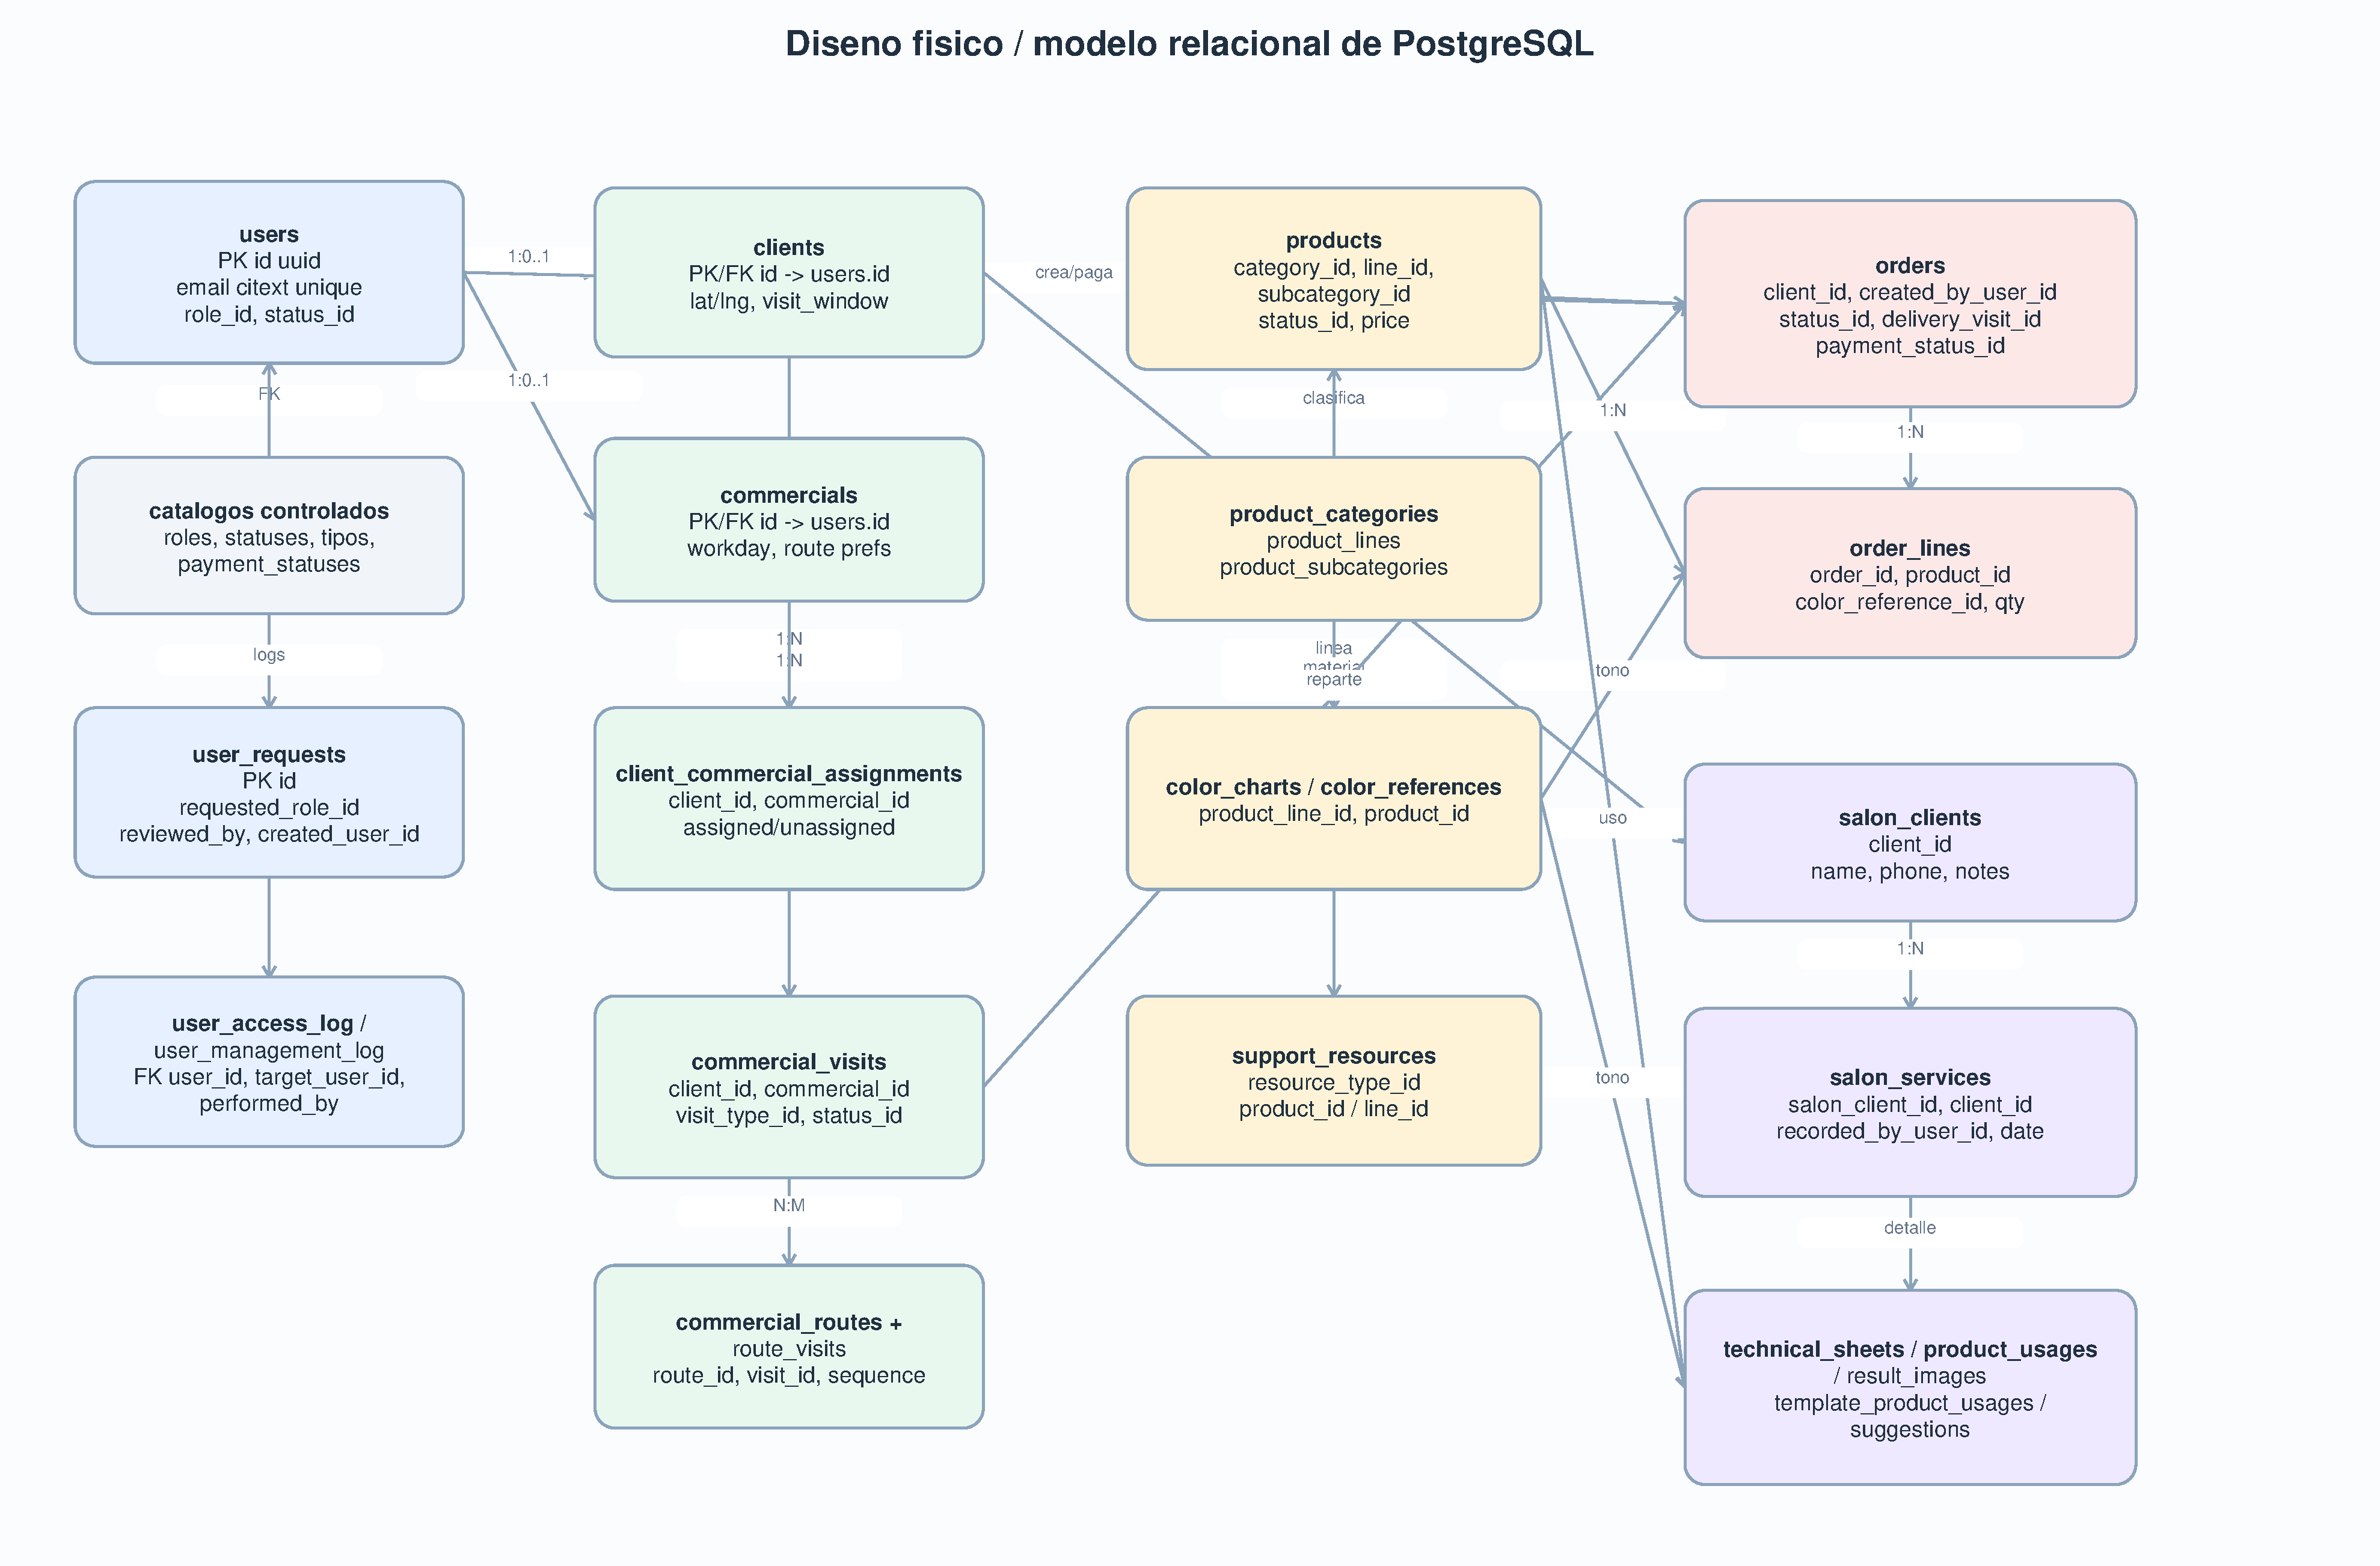
\includegraphics[width=\linewidth]{./figures/UML/MCD/postgresql-physical-model.pdf}
    \caption{Diseño físico / modelo relacional de PostgreSQL}
    \label{fig:postgresql-physical-model}
\end{figure}

\subsubsection*{Activos multimedia externos}

Las imágenes no se almacenan como binarios en la base de datos. En su lugar, la aplicación delega su gestión en \texttt{Cloudinary} \citep{cloudinaryupload2026}. Esta decisión afecta actualmente a dos familias de activos:

\begin{itemize}
    \item imágenes de perfil de usuarios;
    \item imágenes de catálogo, incluyendo líneas, subcategorías, productos, cartas de color y referencias cromáticas;
    \item imágenes del resultado final de servicios técnicos registrados en el salón.
\end{itemize}

En la base de datos solo se persisten las URLs finales y, cuando procede, metadatos auxiliares como la miniatura asociada a una referencia cromática. Esto simplifica el modelo, reduce el peso de la base de datos y permite reutilizar un almacenamiento optimizado para contenido multimedia.

\subsubsection*{Datos derivados o reconstruibles}

Existen además varios artefactos que la aplicación no persiste como entidad independiente:

\begin{itemize}
    \item el QR del pedido, que se reconstruye a partir del identificador del pedido y se representa mediante \texttt{QuickChart} \citep{quickchartqr2026};
    \item la geometría de ruta comercial, que se consulta a \texttt{OSRM} en tiempo de ejecución \citep{osrmdocs2026};
    \item la geocodificación de una dirección, que se obtiene desde \texttt{Nominatim} cuando hace falta confirmar o recalcular coordenadas \citep{nominatimapi2026};
    \item la ETA visible para cliente, que se calcula a partir de visitas reales, reglas horarias y posición en ruta, y no como un dato fijo aislado.
\end{itemize}

Esta separación evita almacenar resultados efímeros o fácilmente regenerables cuando su valor depende de datos del negocio ya presentes en el sistema.

\subsubsection*{Criterios de diseño adoptados}

La estrategia de almacenamiento aplicada en el proyecto responde a cuatro criterios:

\begin{itemize}
    \item mantener el dato estructurado y transaccional dentro de la base de datos relacional;
    \item externalizar los binarios y recursos multimedia a un servicio especializado;
    \item recalcular bajo demanda la información derivada cuando sea más robusto que persistirla;
    \item limitar el número de entidades persistentes a las que realmente aportan valor al modelo de negocio implementado.
\end{itemize}

Por ello, aunque el sistema ya muestra QR, ETA, mapas, capturas de cámara o recursos externos, no todo ello debe interpretarse como nuevas entidades almacenadas. La memoria debe distinguir entre datos persistidos, activos referenciados e información operativa calculada en el momento.
